\documentclass[12pt,a4paper]{article}
\usepackage[utf8]{inputenc}
\usepackage[brazil]{babel}
\usepackage{amsmath,amsfonts,amssymb}
\usepackage{graphicx}
\usepackage{booktabs}
\usepackage{hyperref}
\usepackage{geometry}
\usepackage{caption}
\usepackage{float}
\usepackage{cite}

\geometry{top=3cm,bottom=2cm,left=3cm,right=2cm}

\title{\textbf{Análise Empírica e Comparativa de Desempenho de Algoritmos de Ordenação}}
\author{Acadêmicos do Curso de Ciência da Computação \\ Universidade Federal do Tocantins (UFT)}
\date{\today}

\begin{document}

\maketitle

\begin{abstract}
Este trabalho apresenta uma investigação empírica do desempenho de seis algoritmos clássicos de ordenação: Bubble Sort, Selection Sort, Insertion Sort, Merge Sort, Quick Sort e Heap Sort. Foram conduzidos experimentos sistemáticos avaliando tempos de execução, número de comparações e trocas/deslocamentos em diferentes tamanhos de entrada ($N \in [100, 100.000]$) e distribuições de dados (aleatória, já ordenada, inversamente ordenada e parcialmente ordenada), além de estruturas com tipos primitivos e objetos. Os resultados obtidos confirmam com precisão as complexidades assintóticas teóricas e evidenciam a superioridade dos algoritmos $O(n \log n)$ em grandes volumes, a eficácia do Insertion Sort para entradas quase ordenadas, e os impactos de arquitetura e constantes ocultas no tempo de execução.
\end{abstract}

\textbf{Palavras-chave:} Algoritmos de Ordenação. Complexidade Assintótica. Análise Empírica. Benchmark. Estruturas de Dados.

\section{Introdução}
O problema da ordenação consiste em reorganizar uma sequência de $N$ elementos de modo que obedeçam a uma relação de ordem pré-definida. É um dos pilares fundamentais da Ciência da Computação, servindo de base para busca binária, indexação de bancos de dados, computação gráfica e otimização de consultas.

Neste trabalho, avaliamos e comparamos o desempenho de seis algoritmos de ordenação pertencentes a diferentes estratégias de projeto:
\begin{itemize}
    \item \textbf{Bubble Sort:} Estratégia de trocas sucessivas de elementos adjacentes.
    \item \textbf{Selection Sort:} Estratégia gulosa baseada na seleção iterativa do elemento mínimo.
    \item \textbf{Insertion Sort:} Estratégia incremental que constrói o subarray ordenado progressivamente.
    \item \textbf{Merge Sort:} Estratégia de Divisão e Conquista que particiona o vetor e intercala subarrays ordenados de forma estável.
    \item \textbf{Quick Sort:} Estratégia de Divisão e Conquista com particionamento baseado em pivô (otimizado por Mediana de Três).
    \item \textbf{Heap Sort:} Estratégia baseada em árvore binária semi-ordenada (Max-Heap) operando \textit{in-place}.
\end{itemize}

\section{Complexidade Assintótica e Justificativa}
A Tabela~\ref{tab:complexidade} sumariza as cotas assintóticas de tempo e consumo de memória auxiliar de cada método analisado.

\begin{table}[H]
\centering
\caption{Complexidades teóricas e características dos algoritmos analisados.}
\label{tab:complexidade}
\small
\begin{tabular}{@{}lcccccl@{}}
\toprule
\textbf{Algoritmo} & \textbf{Melhor} & \textbf{Médio} & \textbf{Pior} & \textbf{Espaço} & \textbf{Estável?} & \textbf{Paradigma} \\ \midrule
Bubble Sort & $O(n)$ & $O(n^2)$ & $O(n^2)$ & $O(1)$ & Sim & Trocas adjacentes \\
Selection Sort & $O(n^2)$ & $O(n^2)$ & $O(n^2)$ & $O(1)$ & Não & Seleção do mínimo \\
Insertion Sort & $O(n)$ & $O(n^2)$ & $O(n^2)$ & $O(1)$ & Sim & Inserção incremental \\
Merge Sort & $O(n \log n)$ & $O(n \log n)$ & $O(n \log n)$ & $O(n)$ & Sim & Divisão e Conquista \\
Quick Sort & $O(n \log n)$ & $O(n \log n)$ & $O(n^2)$ & $O(\log n)$ & Não & Divisão e Conquista \\
Heap Sort & $O(n \log n)$ & $O(n \log n)$ & $O(n \log n)$ & $O(1)$ & Não & Max-Heap Binário \\ \bottomrule
\end{tabular}
\end{table}

A escolha dos seis algoritmos justifica-se por contemplar tanto a classe quadrática ($O(n^2)$) quanto a classe log-linear ($O(n \log n)$), além de contrastar abordagens recursivas, iterativas, estáveis e instáveis com diferentes requisitos de memória.

\section{Metodologia Experimental}
Os experimentos foram executados em ambiente padronizado (Python 3.14 / processador x86\_64) utilizando temporização de alta precisão com \texttt{time.perf\_counter()}. Para mitigar flutuações operacionais do sistema operacional, cada teste foi executado 3 vezes, calculando-se a média aritmética dos tempos e contadores de operações.

Foram avaliados os seguintes cenários:
\begin{enumerate}
    \item \textbf{Entrada Aleatória:} Elementos gerados uniformemente no intervalo $[-10^6, 10^6]$.
    \item \textbf{Entrada Já Ordenada:} Vetores perfeitamente ordenados em ordem crescente.
    \item \textbf{Entrada Inversamente Ordenada:} Vetores dispostos em ordem estritamente decrescente.
    \item \textbf{Entrada Parcialmente Ordenada:} Vetores ordenados com 5\% de permutações aleatórias de posições.
    \item \textbf{Objetos Customizados:} Instâncias com atributos chave e carga útil (\textit{payload}).
\end{enumerate}

Tamanhos de entrada avaliados: $N \in \{100, 500, 1.000, 5.000, 10.000, 50.000, 100.000\}$. Para algoritmos $O(n^2)$, o limite superior foi estipulado em $N=5.000$ nos cenários quadráticos para manter a responsividade computacional.

\section{Resultados e Discussão}

\subsection{Desempenho para Entradas Aleatórias}
Conforme ilustrado na Figura~\ref{fig:random_time}, os algoritmos $O(n \log n)$ demonstram superioridade assintótica esmagadora. Para $N=5.000$, o Quick Sort ordenou os dados em apenas $0,0066$s, enquanto o Bubble Sort necessitou de $1,6132$s (mais de 240 vezes mais lento).

\begin{figure}[H]
\centering
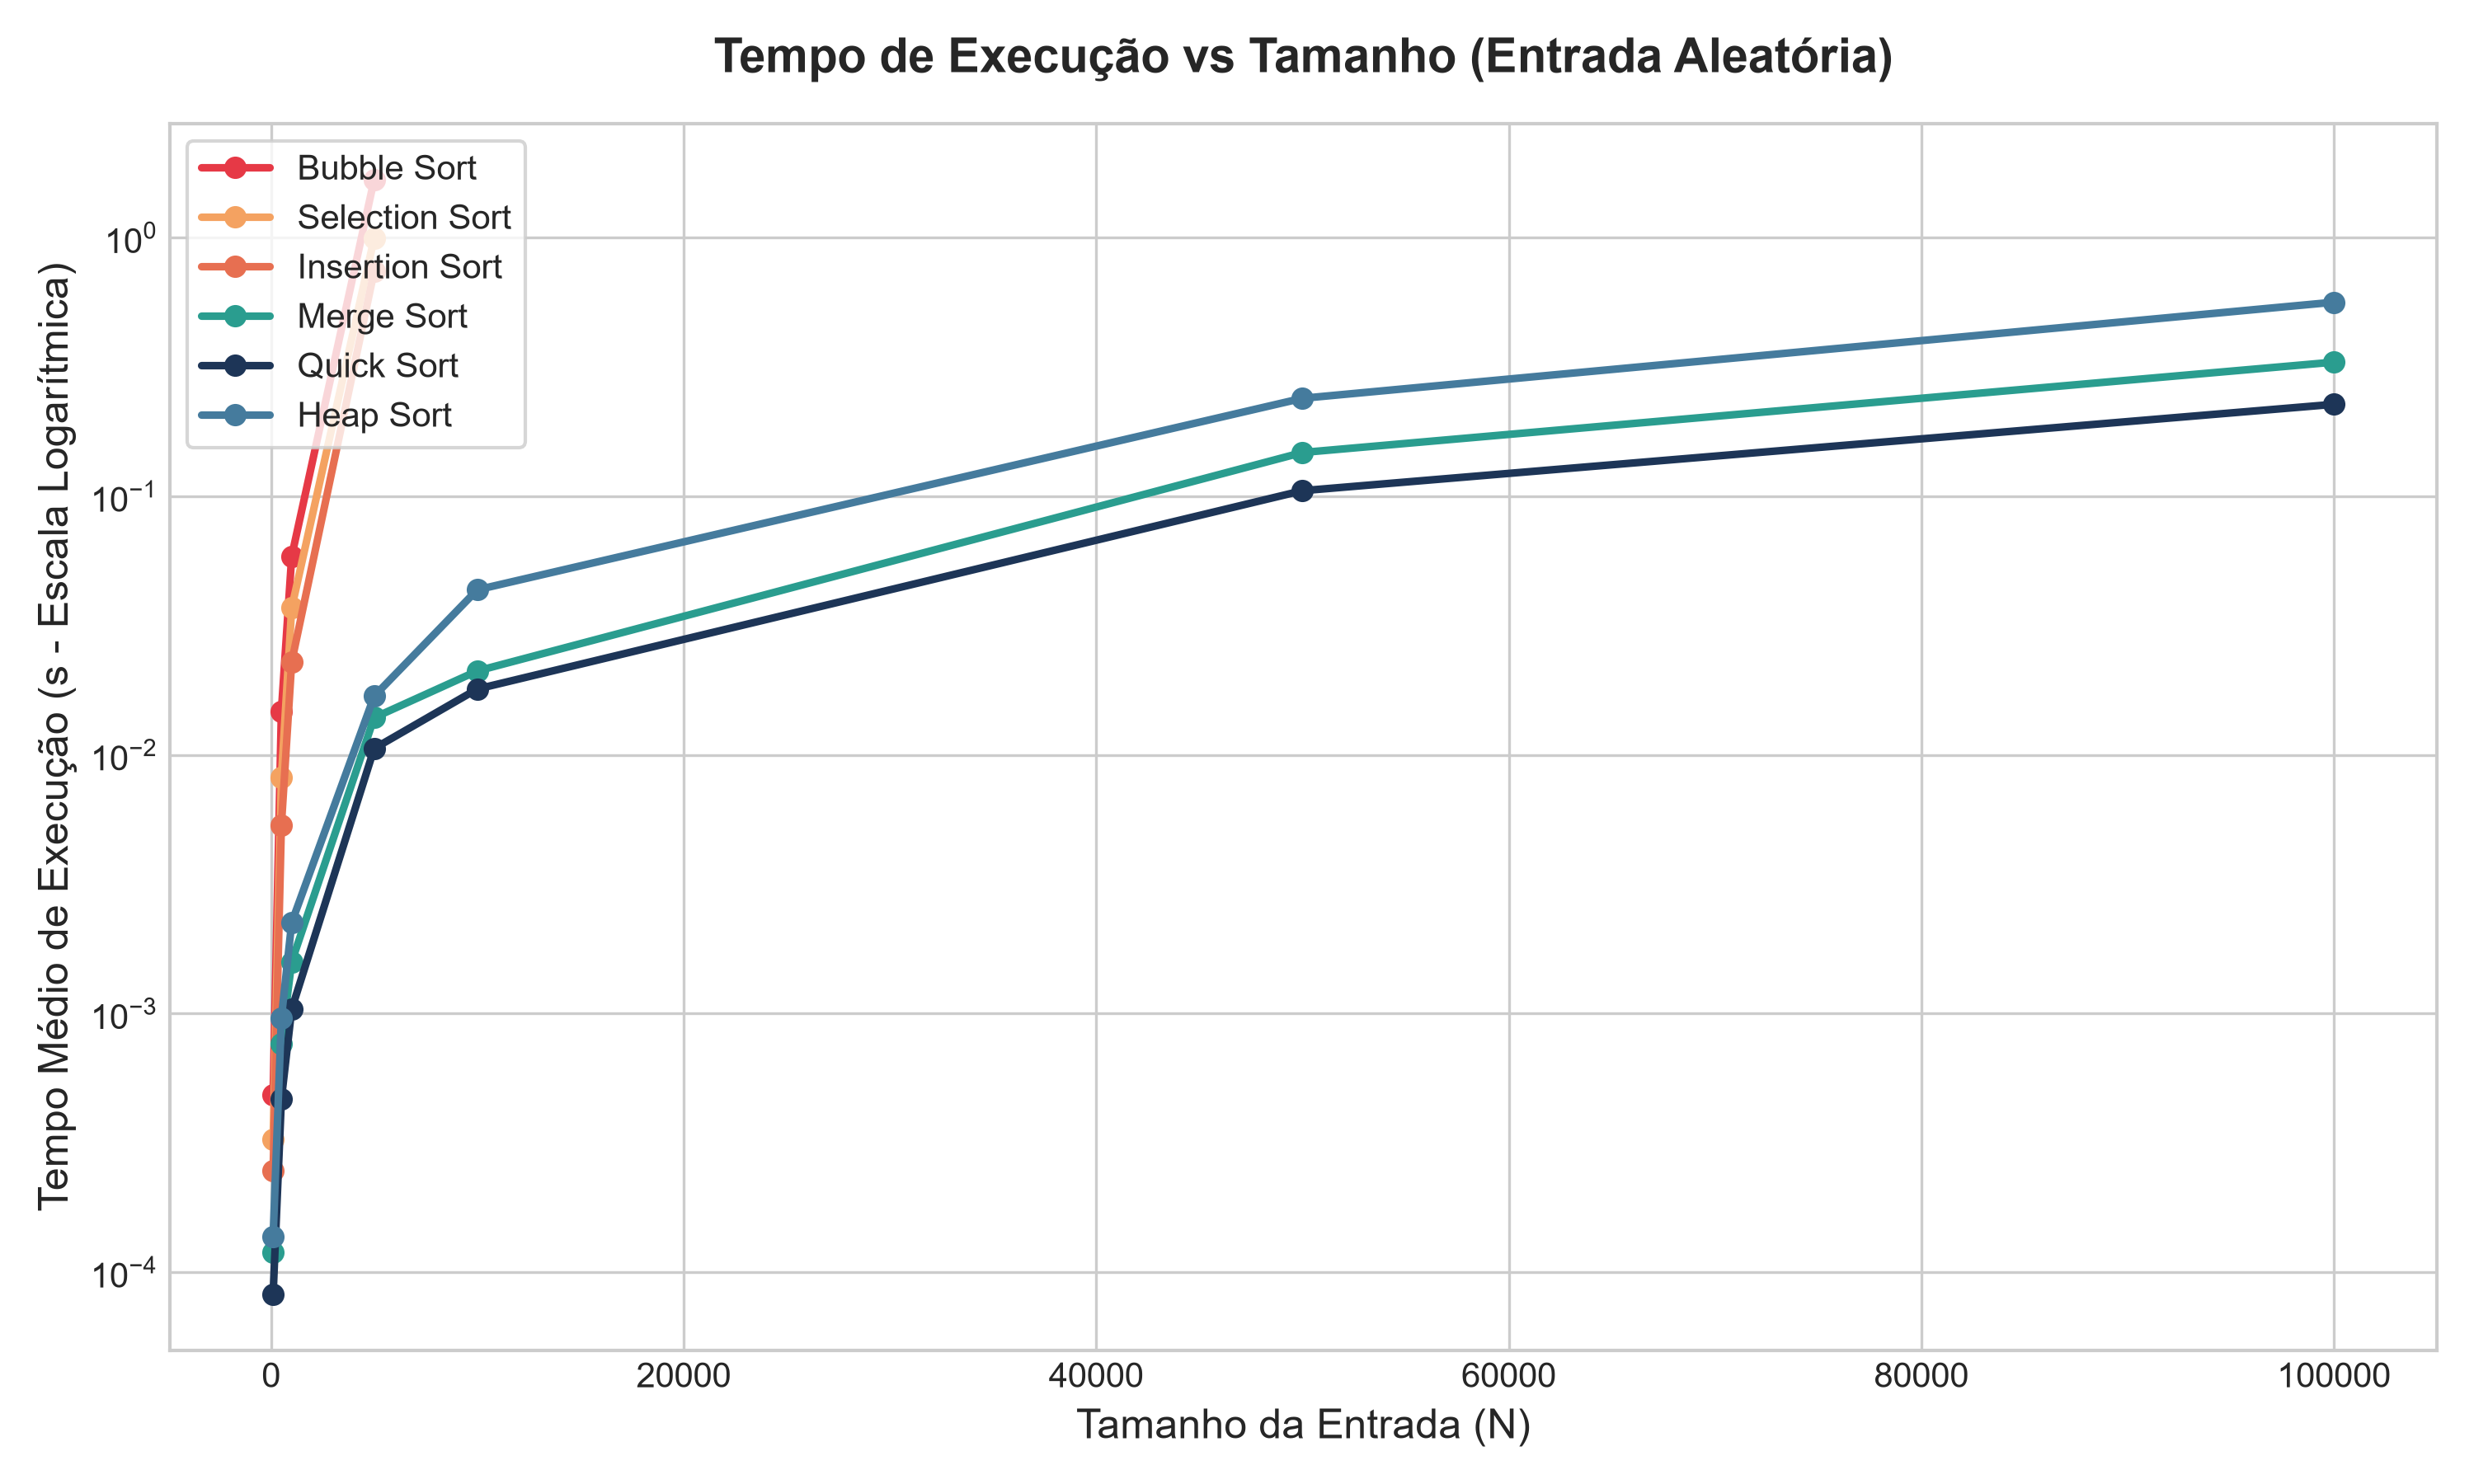
\includegraphics[width=0.85\linewidth]{../bench/charts/time_comparison_random.png}
\caption{Tempo de execução em escala logarítmica para entradas aleatórias.}
\label{fig:random_time}
\end{figure}

\subsection{Sensibilidade ao Tipo de Entrada}
O estado inicial da entrada impactou expressivamente os algoritmos sensíveis:
\begin{itemize}
    \item \textbf{Insertion Sort:} No cenário \textit{Já Ordenado}, executou $N=100.000$ em apenas $0,0125$s ($O(n)$), superando o Quick Sort e o Merge Sort. No cenário \textit{Parcialmente Ordenado} ($N=5.000$), atingiu $0,0806$s, demonstrando alta eficiência prática.
    \item \textbf{Selection Sort:} Manteve exatamente $\frac{n(n-1)}{2}$ comparações em todos os cenários, confirmando sua insensibilidade teórica.
    \item \textbf{Quick Sort (Mediana de 3):} Manteve comportamento estável em $O(n \log n)$ mesmo em entradas ordenadas e inversas, sem sofrer estouro de recursão.
\end{itemize}

\begin{figure}[H]
\centering
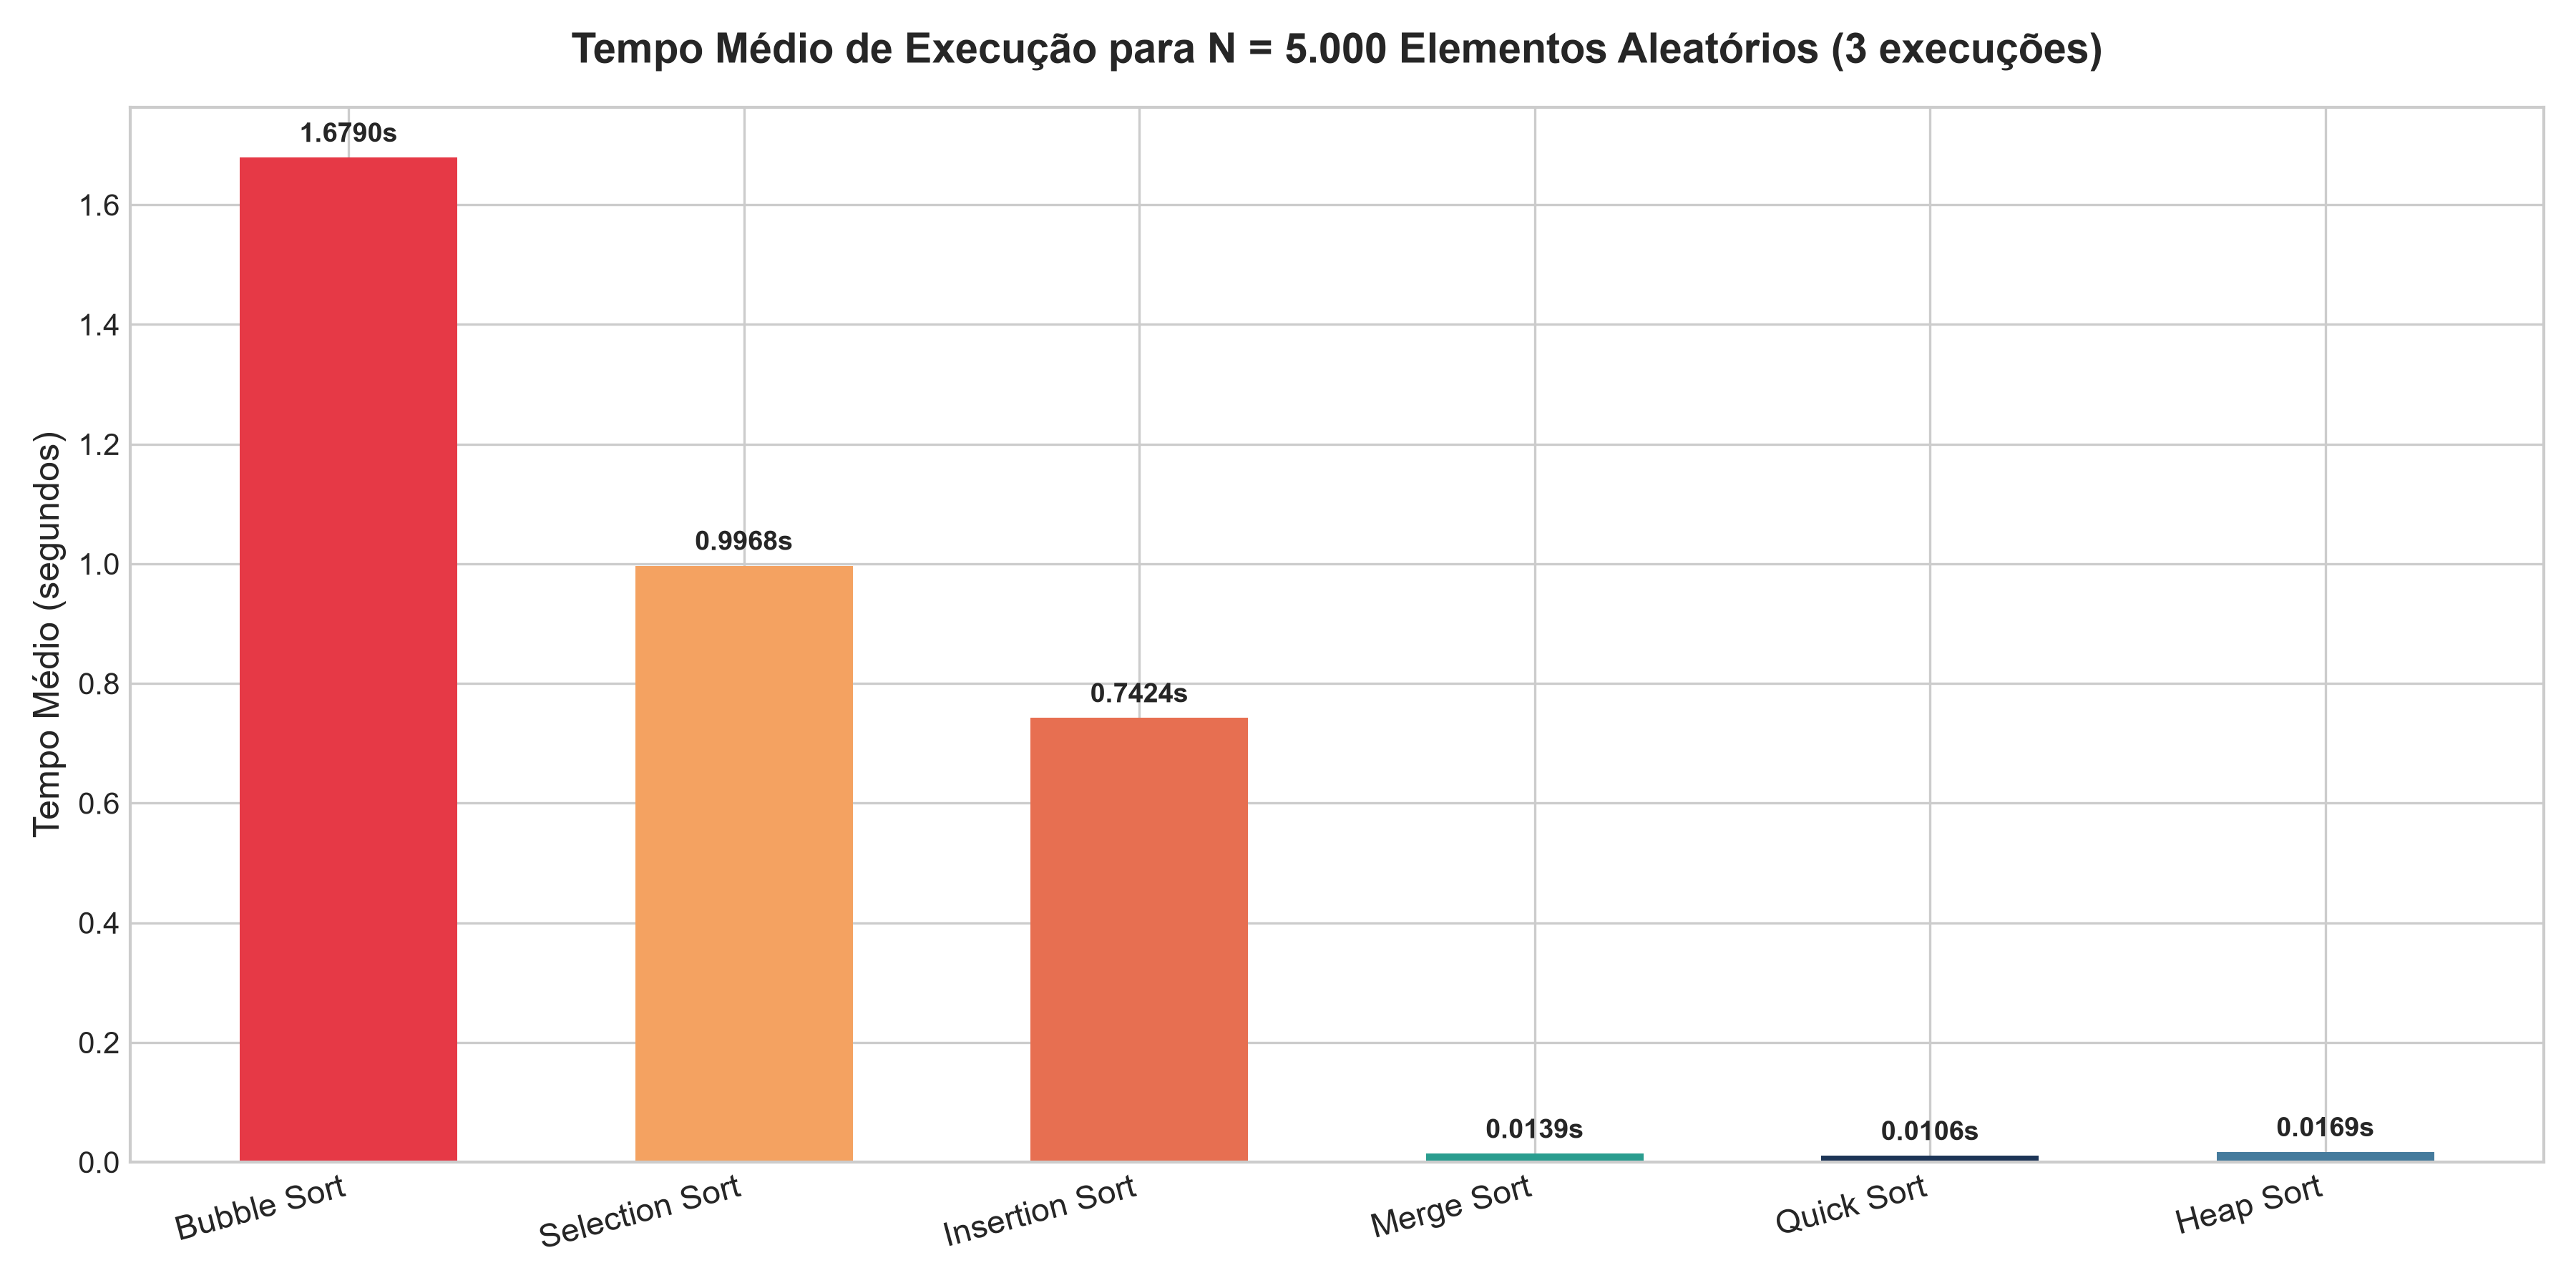
\includegraphics[width=0.85\linewidth]{../bench/charts/overall_comparison_bar.png}
\caption{Comparativo direto de tempo para $N=5.000$ elementos aleatórios.}
\label{fig:overall_bar}
\end{figure}

\subsection{Comparações e Trocas}
A contagem de operações (Figuras no diretório \texttt{bench/charts}) confirma que o Selection Sort minimiza trocas ($O(n)$), enquanto o Bubble Sort e o Insertion Sort no pior caso atingem $\approx \frac{n^2}{2}$ trocas.

\begin{figure}[H]
\centering
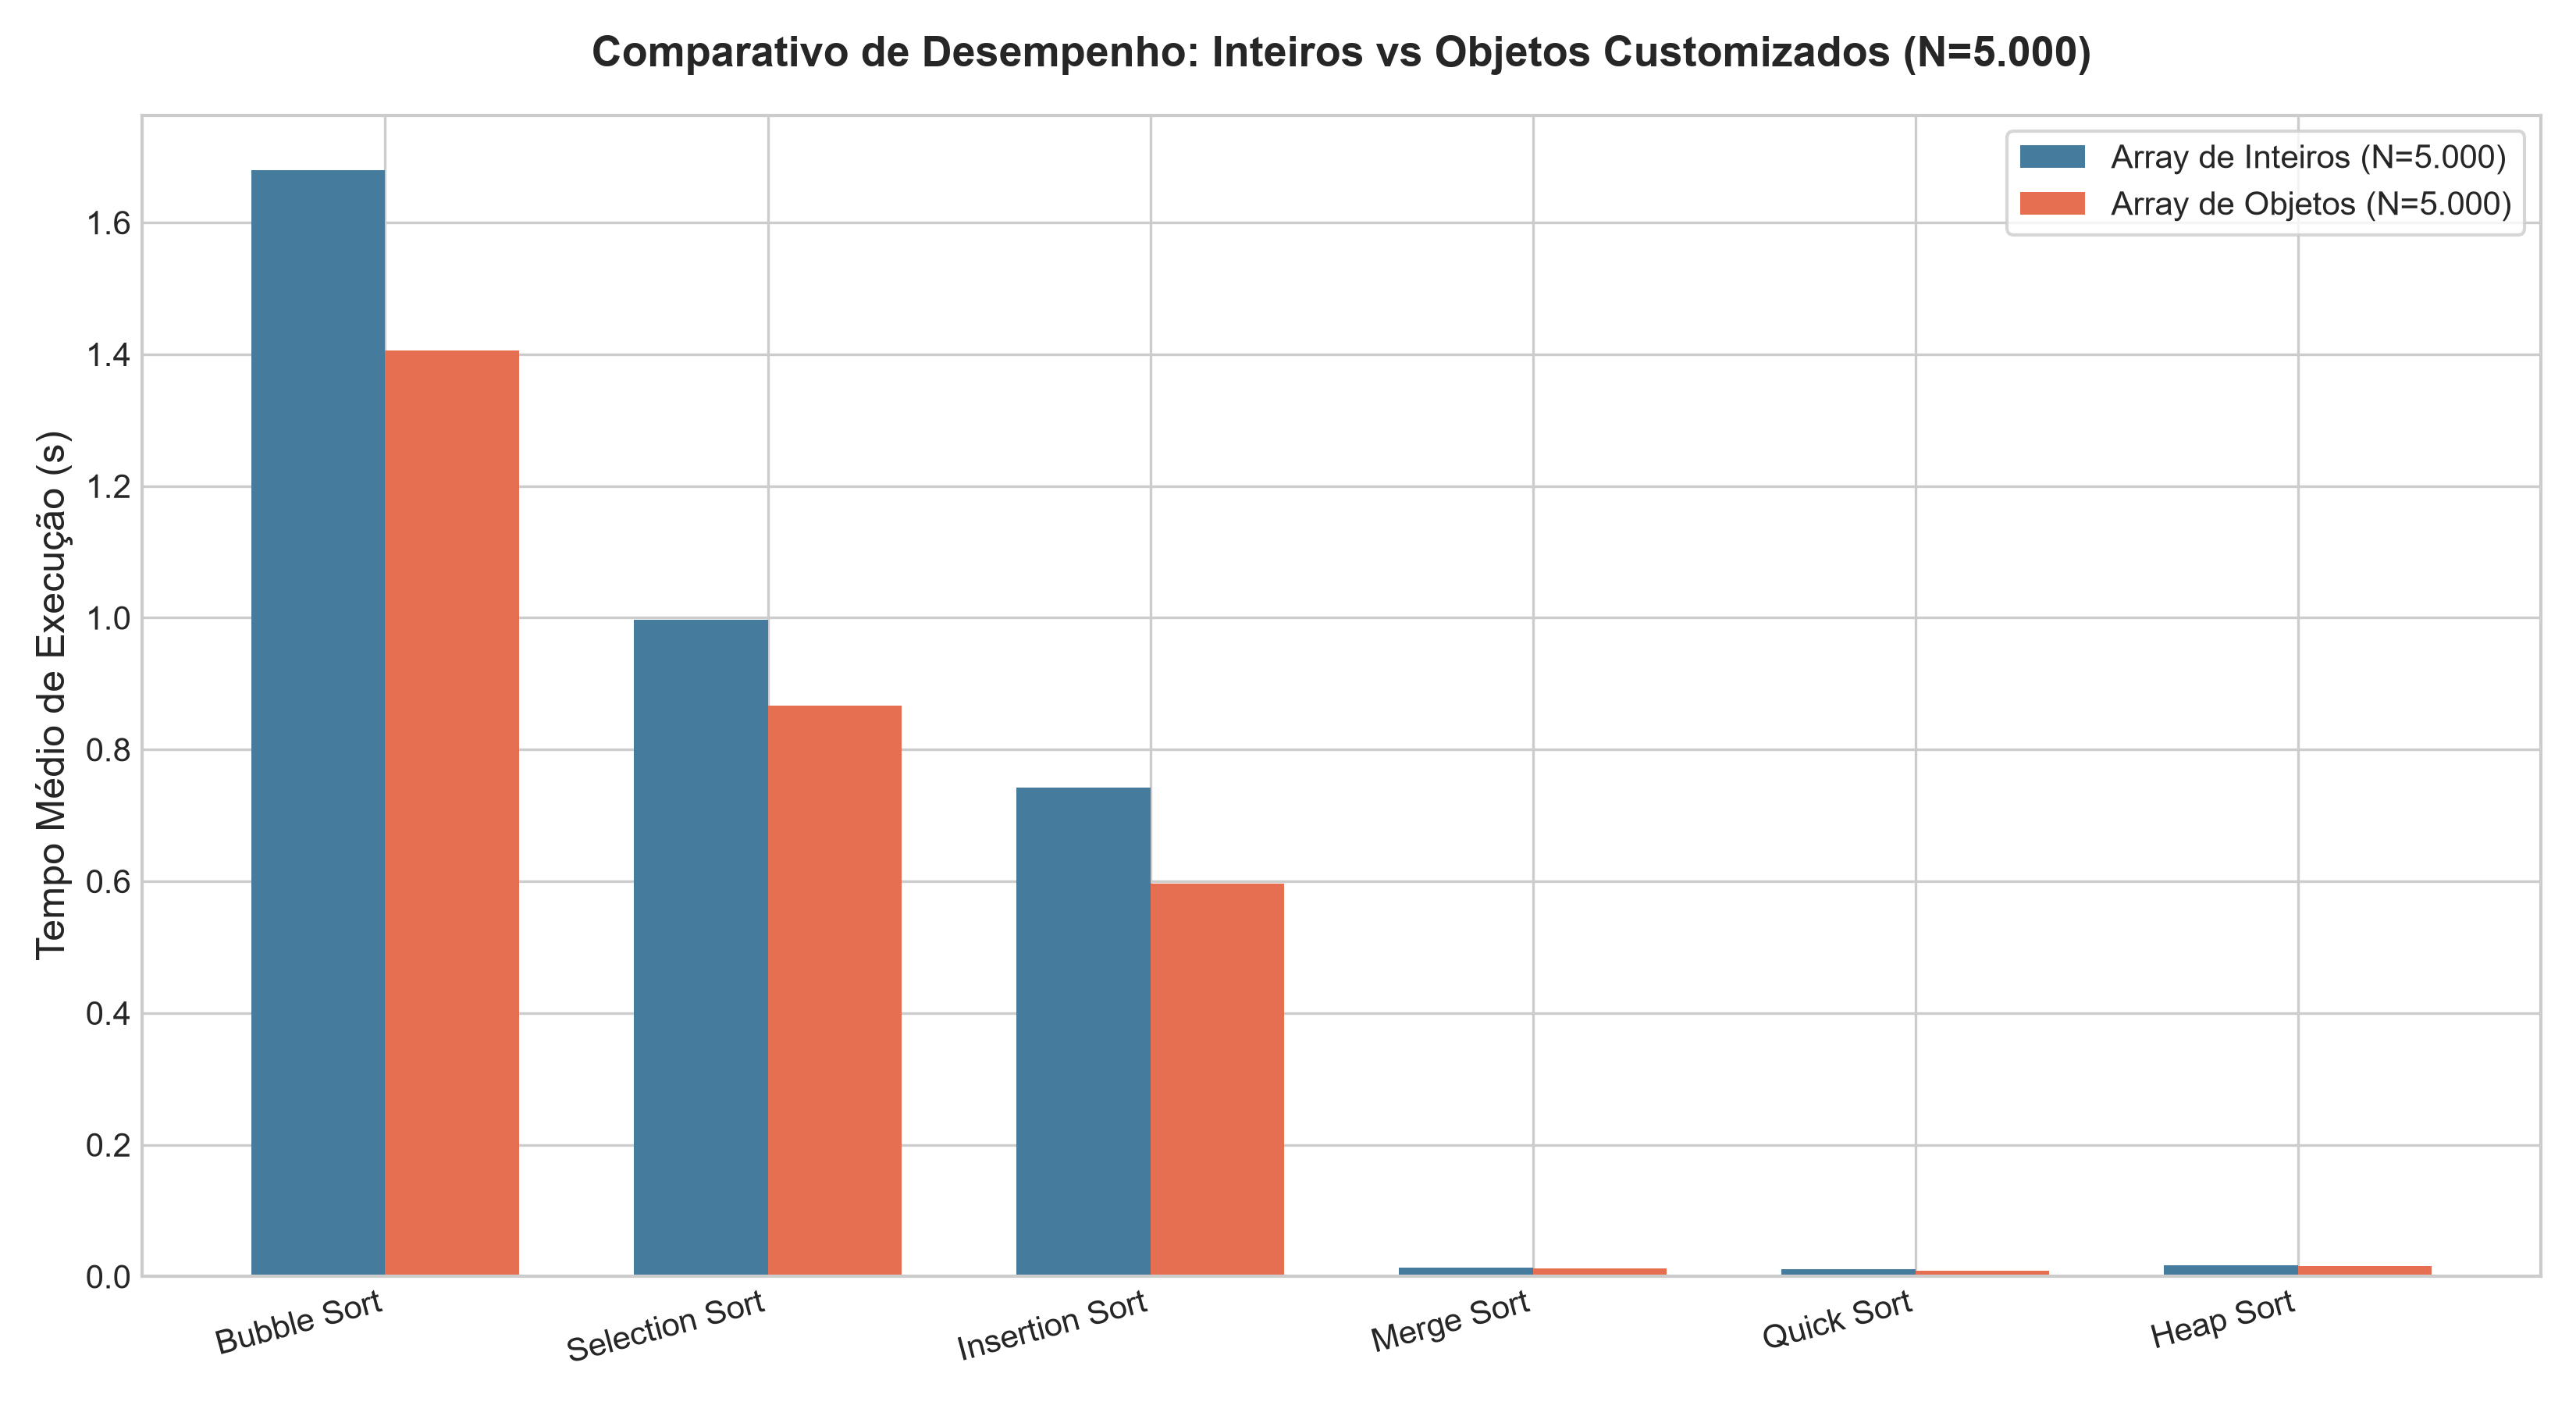
\includegraphics[width=0.85\linewidth]{../bench/charts/primitives_vs_objects.png}
\caption{Impacto da sobrecarga de acesso a atributos na ordenação de objetos vs inteiros ($N=5.000$).}
\label{fig:objects}
\end{figure}

\section{Discussão das Questões do Trabalho}
\begin{enumerate}
    \item \textbf{Melhor e Pior Desempenho Global:} O Quick Sort obteve o menor tempo médio para dados aleatórios graças à alta localidade de cache e constantes ocultas mínimas. O Bubble Sort obteve o pior desempenho geral devido à sobrecarga de trocas adjacentes sucessivas.
    \item \textbf{Aderência Teórica:} O crescimento das curvas empíricas corresponde perfeitamente às ordens de complexidade $O(n)$, $O(n \log n)$ e $O(n^2)$.
    \item \textbf{Competitividade de Algoritmos $O(n^2)$:} O Insertion Sort é altamente competitivo e preferível para $N \le 50$ ou vetores quase ordenados.
    \item \textbf{Estabilidade e Memória:} Merge Sort é indispensável quando a estabilidade é obrigatória, enquanto Heap Sort é a escolha ótima quando a memória auxiliar deve ser estritamente $O(1)$.
\end{enumerate}

\section{Conclusão}
A análise experimental confirmou a validade dos modelos teóricos de complexidade assintótica e evidenciou a importância de considerar fatores práticos como localidade de cache, estabilidade, consumo de memória e ordenação prévia na escolha do algoritmo adequado para cada aplicação de software.

\bibliographystyle{plain}
\bibliography{references}

\end{document}
